
\documentclass[12pt,letterpaper,notitlepage]{report}

\usepackage{graphicx}

\usepackage{natbib}

\usepackage[T1]{fontenc}

\usepackage{ucs}

\usepackage[utf8x]{inputenc}

\usepackage[spanish]{babel}

\usepackage{helvet}

\usepackage{url}

\usepackage{sectsty}

\usepackage{amsmath}

\usepackage[small,sf]{caption}

\setlength{\oddsidemargin}{0. true cm}

\setlength{\evensidemargin}{0. true cm}

\setlength{\protect\textwidth}{16.5 true cm}

\setlength{\topmargin}{0.5 true cm}

\setlength{\textheight}{20 true cm}

\newcommand{\ie}{{\em i.e.  }}  \newcommand{\eg}{{\em e.g.  }}

\newcommand{\txh}{\textheight}

\newcommand{\txw}{\textwidth}

\newcommand{\scrsz}{\scriptsize}

\newcommand{\mc}[3]{\multicolumn{#1}{#2}{#3}}

\newcommand{\Cpp}{{\bfseries C++}}

\DeclareMathOperator{\Tr}{Tr}


% Some commands to handle linespacing

\newlength{\spacing} \setlength{\spacing}{\baselineskip}

\newcommand{\nspace}[1]{\setlength{\baselineskip}{#1\spacing}}
\newenvironment{linespacing}[1]{\nspace{#1}}{}

\allsectionsfont{\sffamily}

\bibliographystyle{apalike}


\title{Manual de usuario del programa\\ \emph{Detección de Esquinas}.}

\author{Dr. Arturo Espinosa Romero\\ Dr. Ricardo Legarda Sáenz\\
  Dr. Aaron Aguayo}

\date{}

\begin{document}
 {\sffamily

 \maketitle

\begin{linespacing}{1.5}

\section{Introducción}

Este programa se utiliza como  un apoyo didáctico en el curso ``Visión
Computacional''  que  se  imparte  a  alumnos de  la  Licenciatura  en
Ingeniería  en  Computación  en  la  Facultad  de  Matemáticas  de  la
Universidad Autónoma de Yucatán.

En  particular este  material sirve  como apoyo  en la  unidad  seis del
programa  en donde  se es necesario entender métodos que permitan
determinar las regiones de interés a se procesadas en la busque da
correspondencias entre imágenes, adicionalmente se muestran técnicas
eficientes para la . Este programa  tiene  aparte otro componente
importante y es el que ilustra técnicas para el cómputo eficiente de
sumatorias sobre imágenes, a través del uso de uso de matrices de
acumulación. Y por último tiene un elemento  didáctico,  pues
demuestra  el estilo de  programación que se debe usar  al programar
utilizando la biblioteca OpenCV, y como compilar el código. 

Este programa tiene como objetivo presentar al estudiante el detector
de esquinas de ~\citet{Harris+Stephens1988}. El detector de esquinas de Harris
se utiliza principalmente para la detección de regiones de interés en las
imágenes. Por región de interés entendemos aquella en donde hay
variaciones locales de intensidad de la imagen cuyo gradiente tenga
componentes ortogonales equivalentes en magnitud, y que esta magnitud
sea lo suficientemente grande. Esto suele ocurrir en regiones donde
dos bordes se intersectan, y se le suele llamar a este tipo de
filtros como detectores de esquinas. En particular aquí se implementa
un método conocido como el detector de esquinas de Harris, este método
calcula a partir de las derivadas parciales de una región
$W(\mathbf{x})$ alrededor de un pixel con coordenadas
$\mathbf{x}=\left[x,y\right]^\top$ un valor escalar que representa la
``esquinidad'' de ese pixel. Dicho computo se obtiene evaluando la
siguiente fórmula: \[C(G) = \det |G| - k \Tr^2 G,\] donde:
\[ G=\left[\begin{array}{cc} \sum_{\tilde{x}} I_x^2(\tilde{x}) &
    \sum_{\tilde{x}} I_x(\tilde{x})I_y(\tilde{x})\\ \sum_{\tilde{x}}
    I_x(\tilde{x})I_y(\tilde{x}) & \sum_{\tilde{x}}I_y^2(\tilde{x}) \end{array}\right],\]
                             
\bigskip
                             
$\tilde{x} \in W(\mathbf{x})$ y $W(\mathbf{x})$ es una ventana de dimensiones $ w \times w$ centrada en la coordenada $\mathbf{x}$. 

El costo computacional de evaluar esta función reside principalmente
en el computo de las derivadas direccionales de la función, y en el
cómputo de la matriz $G$. El computo de las derivadas se hace haciendo
una convolución de la imagen original con la derivada unidimensional
de una función Gaussiana, y se utiliza una técnica basada en el
cómputo de una matriz de acumulación para mantener constante el costo
computacional de calcular la matriz $G$~\citep{Simard+ETAL1999,
  Viola+Jones2004}. Para comparar ambos métodos se realizaron dos
implementaciones, una utilizando la matriz de acumulación
(\verb!DeteccionEsquinasCS.cpp!) y otra que utiliza una sumatoria
convencional sobre la imagen (\verb!DeteccionEsquinasM.cpp!).


\section{Uso}

La interacción con el programa se hace invocándolo desde una emulador de terminal. Primero que hay que ubicarse en el directorio en donde está el archivo ejecutable, e invocarlo como sigue:
\begin{verbatim}
$ DeteccionEsquinasM <Número de cámara>
\end{verbatim}
ó
\begin{verbatim}
$ DeteccionEsquinasCS <Número de cámara>
\end{verbatim}

dependiendo que versión del programa se quiera usar. 

\smallskip

 El programa debe  recibir como único parámetro el número de
 cámara. Al ejecutarse se abre una ventana distribuida como sigue: en
 la parte superior se proporcionan tres controles deslizantes, que nos
 permiten definir tres parámetros de operación: la desviación estándar $\sigma$
 usada para el cómputo de las derivadas direccionales, la constante
 $k$ que determina el comportamiento del detector de esquinas de
 Harris, y por último un control deslizante que controla $w$, el tamaño de
 la ventana que se utiliza para el cómputo de la matriz $G$.
 En la parte inferior de la ventana se muestra un  arreglo de 4 imágenes organizado en un mosaico de $2\times
 2$. La imagen superior izquierda es la imagen tal como es capturada
 por la cámara, y las siguientes imágenes muestran el resultado de
 aplicar diferentes operaciones a la imagen. En la siguiente tabla se
 muestra en orden de izquierda a derecha y arriba abajo las
 operaciones que se despliegan en la ventana de ejecución:
\begin{center}
  \fbox{
    \begin{tabular}{|p{0.45\textwidth}|p{0.45\textwidth}|}\hline
      Imagen original & Magnitud de la primera derivada horizontal\\\hline
      Primera derivada vertical&  valor $C$ de la medida de
      ``esquinidad'' de Harris.\\\hline
    \end{tabular}}
\end{center} mientras que en la figura~\ref{fig:DE} se muestra una
captura de la ventana del programa durante su ejecución.


\begin{figure}[!htbp]
  \centering
  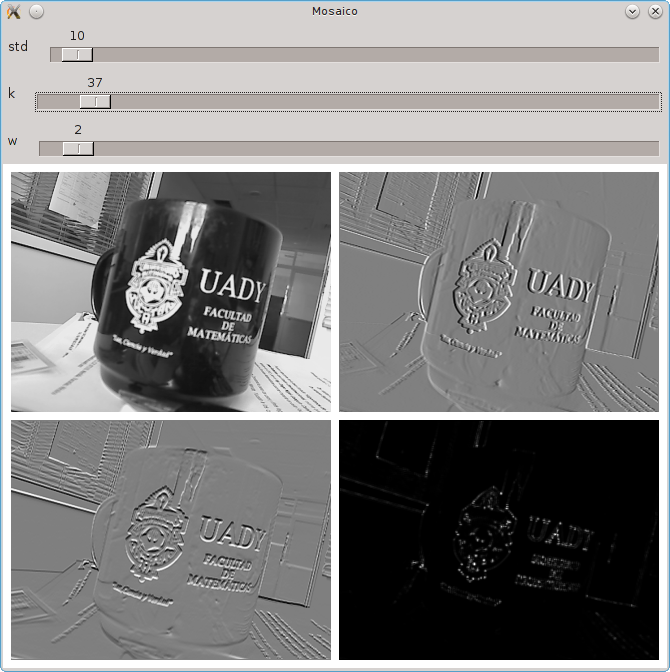
\includegraphics[width=0.9\textwidth]{DeteccionEsquinas.png}
  \caption{Mosaico de imágenes en donde se muestra el funcionamiento del programa.}
\label{fig:DE}
\end{figure}

Durante la ejecución del programa en la consola se imprime el tiempo
en milisegundos que se requiere para realizar el cómputo de cada
cuadro procesado, y cuando se modifican los controles deslizantes se
muestra el cambio a la variable modificada.

\subsection{Compilación.}

 Para compilar únicamente hay que ejecutar el comando \emph{make} en el
directorio del programa, para generar el programa ejecutable.

\subsection{Dependencias.}

El programa depende de las bibliotecas asociadas a \emph{openCV}, y para generar la documentación requiere los programas \emph{doxygen}, y \emph{graphviz}.

\section {Documentación}

 A fin de generar la documentación técnica, únicamente hay que ejecutar el
 comando \emph{doxygen Doxyfile}.
 Se generará documentación la cual quedara almacenada en el directorio
 \emph{Documentacion}, y generará un directorio llamado \emph{html} y
 otro llamado \emph{latex}. En el primero se encuentra la
 documentación del código en formato html, que puede ser consultada
 con cualquier navegador, mientras que en el segundo se encontrara los
 archivos necesario para generar la documentación; únicamente hay que
 entrar a ese directorio y ejecutar el comando \emph{make}.

\end{linespacing}

  \bibliography{biblio} 
}
\end{document}

%%% Local Variables: 
%%% mode: latex
%%% TeX-master: t
%%% End: 
